% ----------------------------------------------------------------------------
% Author: Rayla Kurosaki
% GitHub: https://github.com/rkp1503
% ----------------------------------------------------------------------------

\chapter{Figures}\label{chapter:figures}
\begin{figure}[H]
    \centering
    \begin{subfigure}[b]{0.47\textwidth}
        \centering
        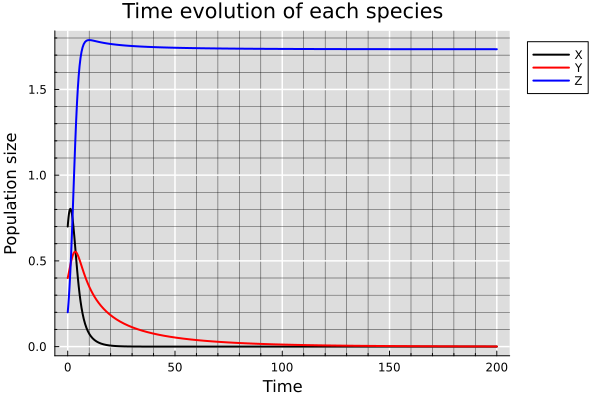
\includegraphics[width=\textwidth]{z_axial.png}
        \caption{$z$-axial equilibria; $r_1 = 0.404$, $r_2 = 0.903$, $p = 0.182$, $\gamma_{12} = 0.639$, $\gamma_{21} = 0.283$, $\gamma_{13} = 0.301$, $\gamma_{31} = 0.110$, $v_1 = 0.645$, $v_2 = 0.175$, $v_3 = 0.145$.}
        \label{fig:z_axial}
    \end{subfigure}
    \hfill
    \begin{subfigure}[b]{0.47\textwidth}
        \centering
        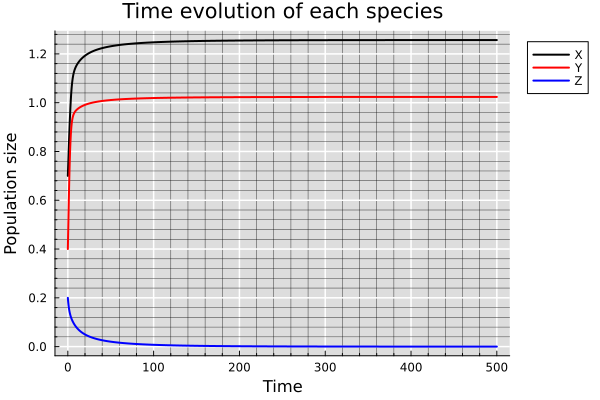
\includegraphics[width=\textwidth]{xy_boundary.png}
        \caption{$xy$-boundary equilibria; $r_1 = 0.978$, $r_2 = 0.613$, $p = 0.326$, $\gamma_{12} = 0.245$, $\gamma_{21} = 0.015$, $\gamma_{13} = 0.920$, $\gamma_{31} = 0.696$, $v_1 = 0.523$, $v_2 = 0.951$, $v_3 = 0.570$.}
        \label{fig:xy_boundary}
    \end{subfigure}
    \hfill
    \begin{subfigure}[b]{0.47\textwidth}
        \centering
        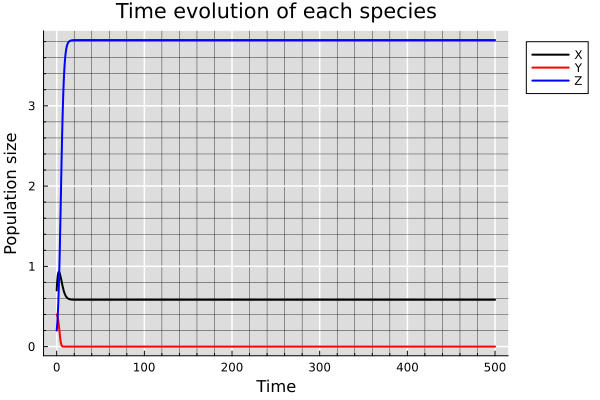
\includegraphics[width=\textwidth]{xz_boundary.png}
        \caption{$xz$-boundary equilibria; $r_1 = 0.102$, $r_2 = 0.763$, $p = 0.271$, $\gamma_{12} = 0.182$, $\gamma_{21} = 0.301$, $\gamma_{13} = 0.109$, $\gamma_{31} = 0.198$, $v_1 = 0.983$, $v_2 = 0.186$, $v_3 = 0.113$.}
        \label{fig:xz_boundary}
    \end{subfigure}
    \hfill
    \begin{subfigure}[b]{0.47\textwidth}
        \centering
        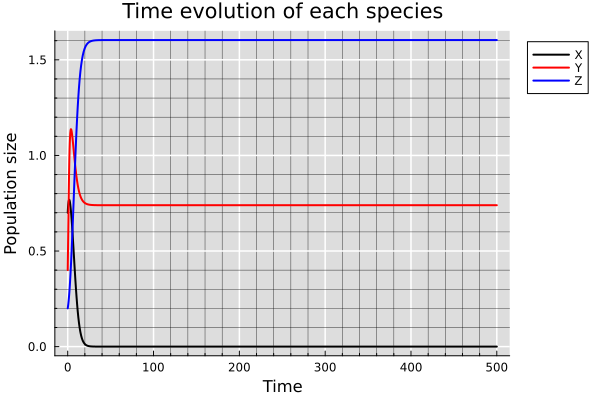
\includegraphics[width=\textwidth]{yz_boundary.png}
        \caption{$yz$-boundary equilibria; $r_1 = 0.978$, $r_2 = 0.310$, $p = 0.843$, $\gamma_{12} = 0.002$, $\gamma_{21} = 0.407$, $\gamma_{13} = 0.859$, $\gamma_{31} = 0.446$, $v_1 = 0.872$, $v_2 = 0.201$, $v_3 = 0.959$.}
        \label{fig:yz_boundary}
    \end{subfigure}
       \caption{Showing the stability of equilibrium points with different set of parameters.}
       \label{fig:semi-trivial-equilibria-plots}
\end{figure}

\begin{figure}[H]
    \centering
    \begin{subfigure}[b]{0.49\textwidth}
        \centering
        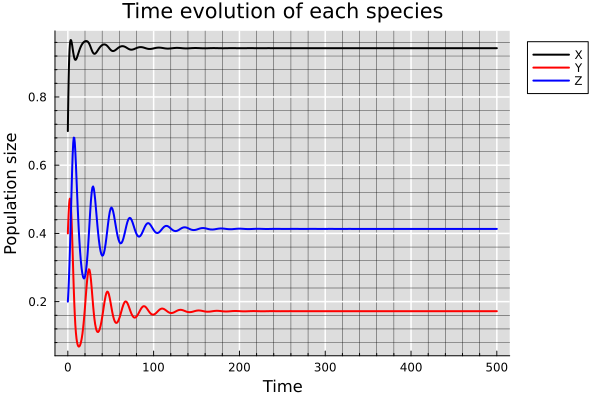
\includegraphics[width=\textwidth]{interior.png}
        \caption{Stability of the interior equilibrium.}
        \label{fig:interior}
    \end{subfigure}
    \hfill
    \begin{subfigure}[b]{0.49\textwidth}
        \centering
        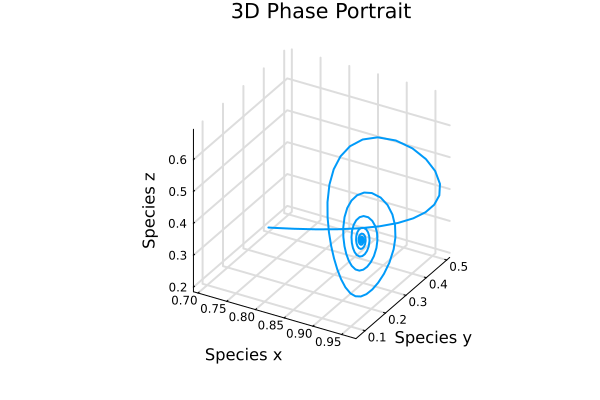
\includegraphics[width=\textwidth]{interior_pp_3D.png}
        \caption{3D phase portrait.}
        \label{fig:phase_plane_3d}
    \end{subfigure}
    \hfill
    \begin{subfigure}[b]{0.49\textwidth}
        \centering
        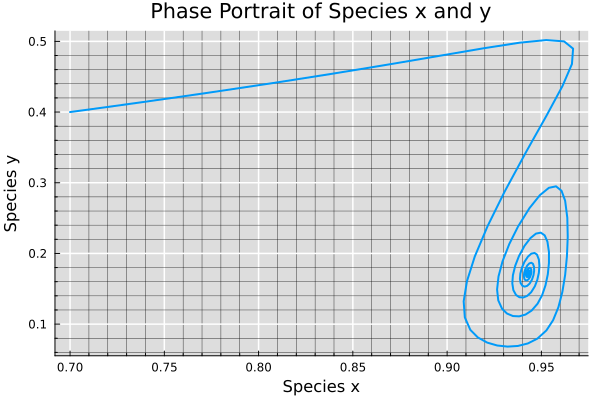
\includegraphics[width=\textwidth]{interior_pp_xy.png}
        \caption{$xy$ phase plane.}
        \label{fig:phase_plane_xy}
    \end{subfigure}
    \hfill
    \begin{subfigure}[b]{0.49\textwidth}
        \centering
        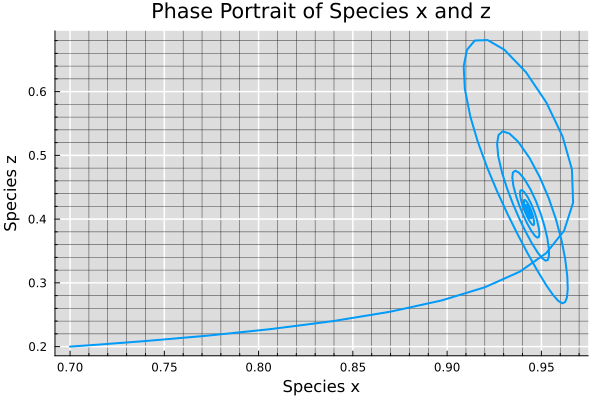
\includegraphics[width=\textwidth]{interior_pp_xz.png}
        \caption{$xz$ phase plane.}
        \label{fig:phase_plane_xz}
    \end{subfigure}
    \hfill
    \begin{subfigure}[b]{0.49\textwidth}
        \centering
        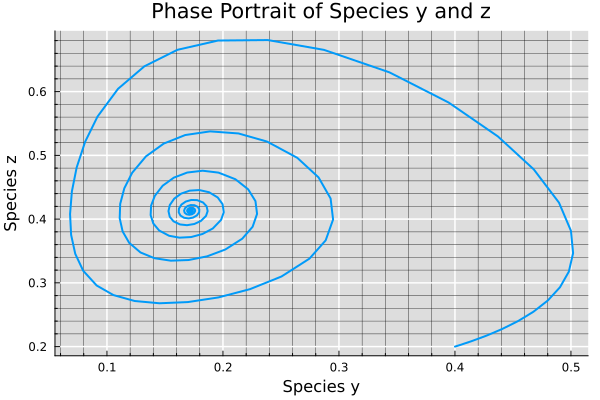
\includegraphics[width=\textwidth]{interior_pp_yz.png}
        \caption{$yz$ phase plane.}
        \label{fig:phase_plane_yz}
    \end{subfigure}
       \caption{Different types of plots to show the behavior of \myref[Model]{model:3.2} where $r_1 = 0.635$, $r_2 = 0.742$, $p = 0.853$, $\gamma_{12} = 0.142$, $\gamma_{21} = 0.002$, $\gamma_{13} = 0.148$, $\gamma_{31} = 0.215$, $v_1 = 0.090$, $v_2 = 0.891$, $v_3 = 0.980$.}
       \label{fig:nontrivial-equilibria-plots}
\end{figure}
